\section*{Problema 2.4}

\textbf{Decidimos que dos observaciones $x_i$ , $x_j$ son conectados por una arista en el grafo correspondiente si $x_i$ está entre los k-vecinos más cercanos de $x_i$ o $x_j$ está entre los k-vecinos más cercanos de $x_i$ . Muestra que la adición de una sola observación en este ejemplo puede destruir por completo el desenrollamiento. Márcala en el dibujo y explícalo.}

\begin{figure}[H]
    \centering
    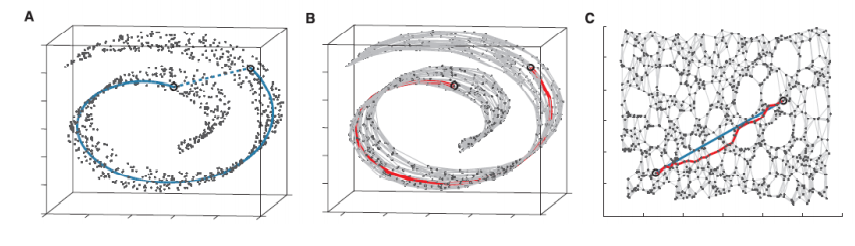
\includegraphics[width=13cm]{Graphics/Problema_2_4.png}
    \caption{Datos originales dados.}
    \label{fig:problema2.4}
\end{figure}

La muestra que se añadiria a los datos mostrados en la figura \ref{fig:problema2.4} es un dato entre la sabada formada. Esto puede ilustrarse en la figura \ref{fig:problema2.4_answer}. Como la figura \ref{fig:problema2.4} esta formada con los k-vecinos más cercanos, al añadirel nuevo dato se contemplarían los vecinos del mismo y en que conjuntos estaría involucrado el mismo. Dando así que la figura formada se desenrolle.

\begin{figure}[H]
    \centering
    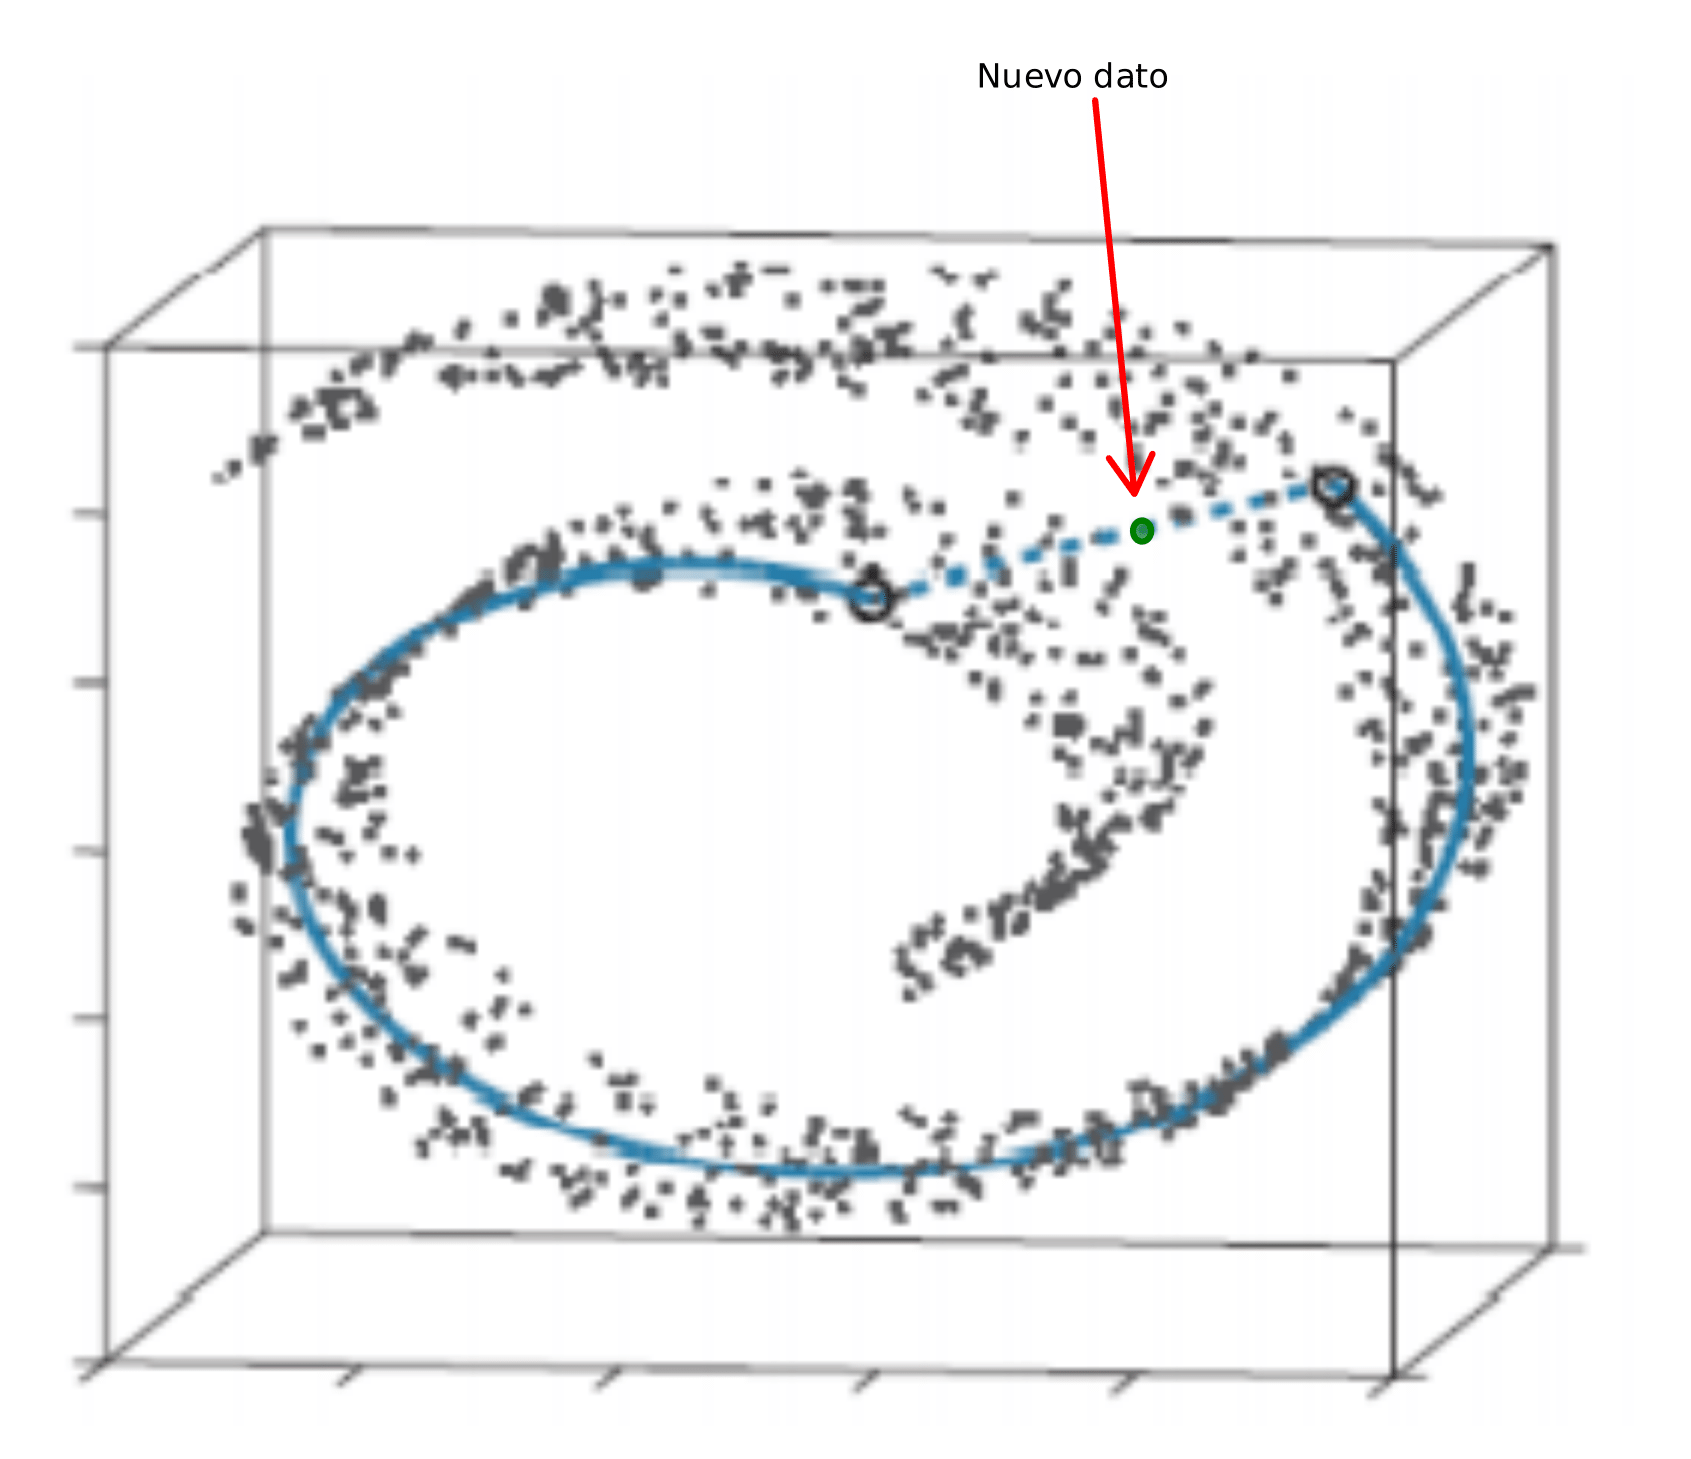
\includegraphics[width=8cm]{Graphics/Problema_2_4_answer.png}
    \caption{Dato propuesto para desenrollar la figura.}
    \label{fig:problema2.4_answer}
\end{figure}